 A trajectory is a function of time $q(t)$ such that $q(t_0)=q_s$ and $q(t_f)=q_g$ (see Trajectory Planning section in \cite{spong}). Trajectory planning expands the path into a 'step-by-step plan' with the introduction of time as a variable, which than could be fed to the controller. Here 'step-by-step' posits the implicit dependency on control frequency, which in case of Panda robot is 1000Hz.
 
 Polynomials of degree n, is a common selection for parametrization of trajectories, where n is dependent on the number of constraints \cite{spong}.Having continuous position, velocity and acceleration (thus no impulsive jerk) for both initial and final configurations lays 6 constraints, so a fifth order polynomial
$$ q(t) = a_0 + a_1t + a_2t^2 + a_3t^3 + a_4t^4 + a_5t^5 $$
would suffice. Taking its derivatives one could reach at:
$$ v(t) = \Dot{q}(t) = a_1 +2 a_2t +3 a_3t^2 +4 a_4t^3 +5 a_5t^4 $$
$$ \alpha(t) = \Ddot{q}(t) = 2 a_2 + 6 a_3t + 12 a_4t^2 + 20 a_5t^3 $$
Plugging $t_0$ and $t_f$ in to above equations and then arranging them in matrix form:
$$\begin{bmatrix}
1 & t_0 & t_0^2 & t_0^3 & t_0^4 & t_0^5 \\
0 & 1 & 2t_0 & 3t_0^2 & 4t_0^3 & 5t_0^4\\
0 & 0 & 2 & 6t_0 & 12t_0^2 & 20t_0^3\\
1 & t_f & t_f^2 & t_f^3 & t_f^4 & t_f^5\\
0 & 1 & 2t_f & 3t_f^2 & 4t_f^3 & 5t_f^4\\
0 & 0 & 2 & 6t_f & 12t_f^2 & 20t_f^3\\ 
\end{bmatrix}
\begin{bmatrix}a_0\\a_1\\a_2\\a_3\\a_4\\a_5\\\end{bmatrix}
=
\begin{bmatrix}q_0\\v_0\\\alpha_0\\q_f\\v_f\\\alpha_f\end{bmatrix}$$
Solving this linear system of equations would result in coefficients $a_i$ that can be used to parametrize the trajectory in the appropriate profiles. These profiles can be seen on Figure \ref{quintics}

 \begin{figure}[ht]
  \centering
  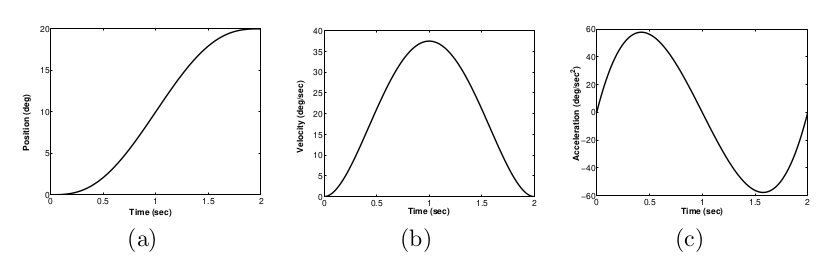
\includegraphics[width=0.45\textwidth]{images/quintics.png}
  \caption{(a) Quintic Polynomial Trajectory. (b) Velocity Profile  (c) Acceleration Profile (figure obtained from \cite{spong}])}
  \label{quintics}
 \end{figure}
